\chapter{Second chapter}
\label{ch:ch2}
The electronic version of the thesis should be made in A4 format (210x297 mm) with one and a half spacing and \textbf{font size 14 Times New Roman}.
The thesis pages should have the following margins: \textbf{left - 25 mm, right - 10 mm, top - 20 mm, bottom - 20 mm.} The paragraph indention must be the same throughout the text and equal to five characters.
\section{Structure of the materials of the thesis}\label{sec:ch2/sec1}

First 5 pages are created automatically in ISU $\Rightarrow$ \textcolor{red}{Table of contents should start at 6 pages:}
{	\color{blue}
	\begin{verbatim}
		\setcounter{page}{6}
	\end{verbatim}
}
%\verb*|\setcounter{page}{6}|

The synopsis in English has the same structure as the synopsis in Russian.
$\Rightarrow$ \textcolor{red}{The counter should be reset before starting synopsis, so that the numbering of Figure and Table is the same  between реферат and synopsis}
{	\color{blue}
	\begin{verbatim}
		\setcounter{figure}{0}
		\setcounter{table}{0}
	\end{verbatim}
}
The main text of the thesis should be divided into chapters using \textbf{no more than three levels} of headings. 

Only using: \verb*|\section{title}| and \verb*|\subsection{title}|
\paragraph*{Tables} should be titled by a caption and numbering.
Tables of each appendix : "Table B.1" if it is given in the Appendix B. 

\paragraph*{Figures} are numbered in Arabic numerals through numbering throughout the synopsis (throughout the thesis).
All figures should be referenced in the text of the thesis. When referencing, it is necessary to write the word \textcolor{red}{Figure} with an indication of its number.
Figures of each appendix: For example, \textcolor{red}{Figure A.3.}

From the реферат to the end of the introduction, the numbering of figures  tables are not attached to the chapter. e.g: \textcolor{red}{Figure 1, Figure 2,} ...
{
	\color{blue}
	\begin{verbatim}
		\counterwithout{figure}{chapter}
		\counterwithout{table}{chapter}
	\end{verbatim}
}
And need to link them when entering the chapter, e.g: Figure \ref{fig:3_1}
{
	\color{blue}
	\begin{verbatim}
		\counterwithin{figure}{chapter}			
		\counterwithout{table}{chapter}	
	\end{verbatim}
}

\paragraph{References} the list of references are made in compliance with \textcolor{red}{GOST 7.0.100.}
{
	\color{blue}
	\begin{verbatim}
		\usepackage[backend=biber, style=gost-numeric]{biblatex}
	\end{verbatim}
}
%\verb*|style=gost-numeric|
\begin{figure}
	\centering
	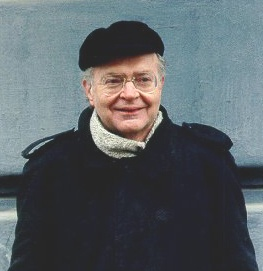
\includegraphics[width=0.4\linewidth]{images/knuth}
	\caption{Knuth}
	\label{fig:3_1}
\end{figure}

\begin{table}
	\centering
	\captionsetup{justification=centering} % выравнивание подписи по-центру
	\caption{Basic SI quantities}%\label{tab:unit:base}
	\begin{tabular}{llc}
		\toprule
		Name 	& 	Command 	& 	Symbol        \\
		\midrule
		Ampere 	 & \verb|\ampere| 	&\si{\ampere}\\
		Candela  & \verb|\candela| 	& \si{\candela} \\
		Kelvin 	 & \verb|\kelvin| 	&\si{\kelvin}\\
		Kilogram & \verb|\kilogram| & \si{\kilogram} \\
		Meter 	 & \verb|\metre| 	&\si{\metre}\\
		Mole 	 & \verb|\mole| 	&\si{\mole}\\
		Second 	 & \verb|\second| 	&\si{\second}\\
		\bottomrule
	\end{tabular}
\end{table}